\clearpage
\subsubsection{Modelado de Adamatzky}

    El modelo de \textit{Physarum polycephalum} de Andrew Adamatzky destaca sus capacidades computacionales. 
        Manipulando \textit{Physarum} con alimentos y repelentes, demuestra la creaci\'on de puertas l\'ogicas y 
        la resoluci\'on de problemas de optimizaci\'on como el camino m\'as corto y el problema del agente viajero \cite{Adamatzky2010}.
        En la Figura \ref{fig:puertas_logicas} se muestra un ejemplo de puertas l\'ogicas creadas por \textit{Physarum}.
    \vskip 0.5cm
    % Imagen 1: Ejemplo de puertas l\'ogicas creadas por Physarum
    \begin{figure}[h]
        \centering
        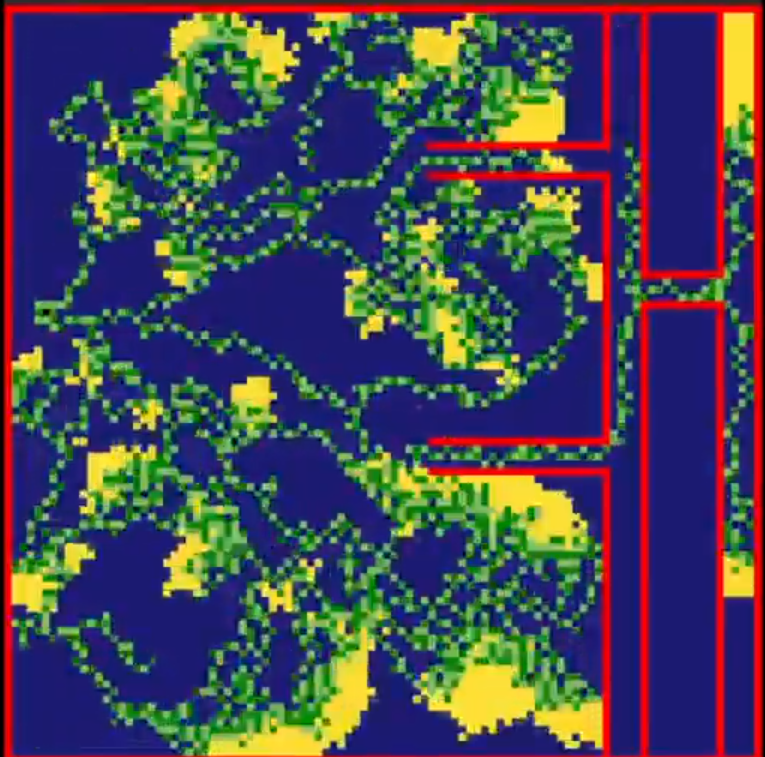
\includegraphics[width=0.5\textwidth]{./images/estado_del_arte/physarum/CompuertasLogicas.png}
        \caption{Ejemplo de puertas l\'ogicas (OR) creadas por \textit{Physarum}.}
        \label{fig:puertas_logicas}
    \end{figure}
    \vskip 0.5cm
    Adamatzky profundiza en la red protoplasm\'atica de \textit{Physarum}, compar\'andola con sistemas humanos, y 
        muestra propiedades memristivas similares a los memristores electr\'onicos \cite{Adamatzky2010}. Su investigaci\'on 
        tambi\'en explora la din\'amica no lineal y la formaci\'on de patrones complejos, significativos para la computaci\'on 
        no convencional \cite{Adamatzky2010}.
    \vskip 0.5cm
    El modelo utiliza part\'iculas de enjambre en un entorno bidimensional (2D) para simular el movimiento ameboide de 
        \textit{Physarum}. Estas part\'iculas tienen etapas sensitiva y motora, interactuando con un quimioatrayente 
        y generando patrones complejos. Adem\'as, se considera la resistencia al movimiento y la influencia de est\'imulos 
        externos como quimioatrayentes y luz, controlando el comportamiento del colectivo.
    \vskip 0.5cm
    Una caracter\'istica destacada es la capacidad del colectivo para cambiar y recuperar su forma, navegar obst\'aculos 
        y dividirse en fragmentos independientes que pueden fusionarse nuevamente, lo cual es deseable en aplicaciones 
        rob\'oticas \cite{Adamatzky2010}. La Figura \ref{fig:adaptacion_obstaculos} ilustra c\'omo el colectivo de 
        \textit{Physarum} se adapta a obst\'aculos.
    \vskip 0.5cm
    % Imagen 2: Colectivo de Physarum adapt\'andose a obst\'aculos
    \begin{figure}[h]
        \centering
        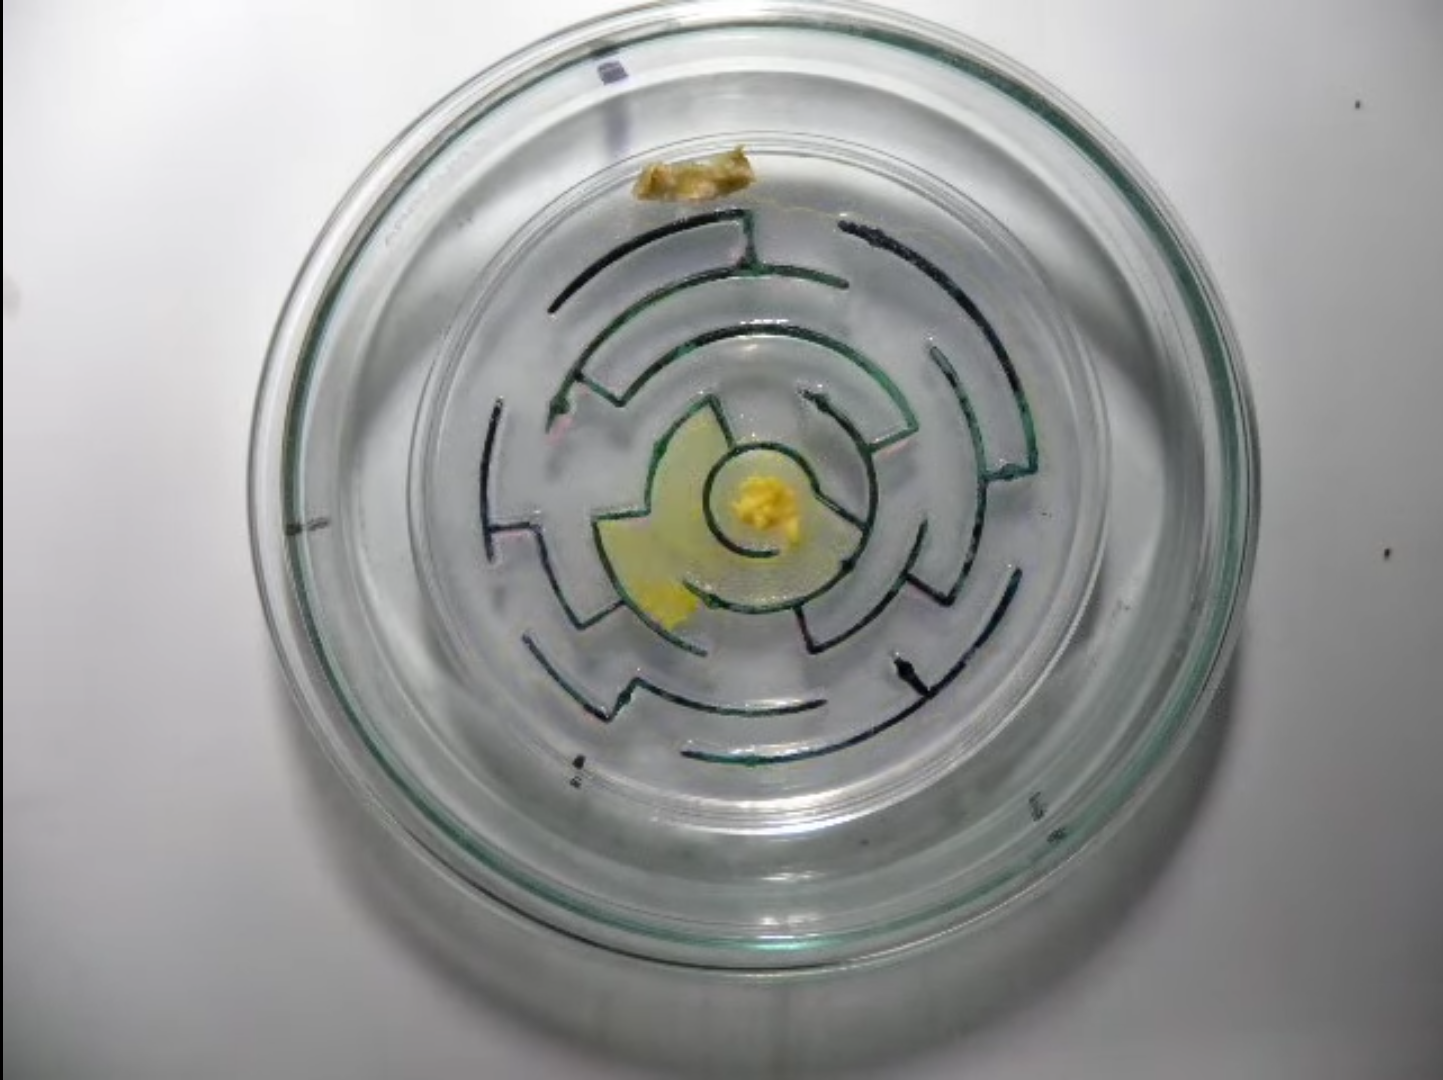
\includegraphics[width=0.5\textwidth]{./images/estado_del_arte/physarum/laberinto.png}
        \caption{Colectivo de \textit{Physarum} adapt\'andose a obst\'aculos. \cite{Adamatzky_2012}}
        \label{fig:adaptacion_obstaculos}
    \end{figure}
    \vskip 0.5cm
    Para m\'as detalles, ver '\textit{Emergence of self-organized amoeboid movement in a multi-
    agent approximation of physarum polycephalum}' \cite{jones2012}.
